\documentclass[12pt,a4paper]{report}
\usepackage[margin=1in]{geometry}
\usepackage{titlesec}
\usepackage{amsmath}
\usepackage{amssymb}
\usepackage[colorlinks=true,urlcolor=black,linkcolor=black]{hyperref}
\usepackage{graphicx}
\usepackage{textcomp}
\usepackage{mathptmx}
\usepackage{tabto,enumitem}
\usepackage{algorithm}
\usepackage{algpseudocode}
\usepackage{wrapfig}

\titleformat{\chapter}{\bf\huge}{\thechapter}{20pt}{\huge\vspace{-.5em}}
    

\begin{document}

\begin{figure}
    \centering
    \begin{center}
    
\includegraphics[width=1.0\linewidth]{Images/concordia_university_system_logo.png}    
    \end{center}
    \label{fig:Concordia University Logo.}
\end{figure}

\title{SOEN 6011\\ Software Engineering Processes\\[3.0em] 

\text{Project Report} \\
\textbf{Function 6 :  $B(x,y)$ Beta Function} \\[1.5em] Supervised By:\\ Dr. Pankaj Kamthan}

\author{Mahavir Nareshbhai Patel (40198619) }
\date{August 05, 2022}


\maketitle

\pagenumbering{roman}
\setcounter{page}{0}

%%%%% Table Of Contents
%\tableofcontents

%%%%% List of Figures
%\listoffigures\addcontentsline{toc}{chapter}{List of Figures}


\chapter{Problem 1}
\pagenumbering{arabic}

\section{Introduction}
The beta function is a special function that belongs to the first category of Euler's integrals. The beta function is denoted by the symbol  "${B}$". $B(x,y)$ refers to the beta function, where $x$ and $y$ are real-valued parameters. \\
The formula of \textbf{$B(x,y)$} is:
    \begin{itemize}
        \item $B(x,y) = \frac{(x-1)! (y-1)!}{(x+y-1)!}$ \text{For positive integers}\cite{1}
        \item $B(x,y)$ = $\int_{0}^{1} {t^{x-1}}{(1-t)^{y-1}} dt$ \text{For positive real numbers}
    \end{itemize}

\section{Properties of Beta Function}
    \begin{itemize}[noitemsep]
        \item Beta function is symmetric which means its beta value is independent of the order of its parameters: $B(x,y) = B(y,x)$
        \item $B(x,y) = B(x,y+1) + B(x+1,y)$
        \item $B(x,y+1) = B(x,y) \cdot [\frac{y}{x+y}]$
        \item $B(x+1,y) = B(x,y) \cdot [\frac{x}{x+y}]$
        \item $B(x,y) . B(x+y,1-y) = \frac{\pi}{x}\sin{\pi y}$
        \item Beta function in terms of Gamma functions as:
            $B(x,y)=\frac{\Gamma x \Gamma y}{\Gamma (x+y)}$ , When x and y are positive whole number then it follows the form of gamma function.
        \item The beta function can be extended to a function with more than two arguments:\\ $B(X_{1},X_{2},...X_{n}) = \frac{\Gamma X_{1} \Gamma X_{2} ... \Gamma X_{n}}{ \Gamma (X_{1} + X_{2} + ... + X_{n})}$
    \end{itemize}

\section{Domain and Co-Domain}
The domains of real numbers are where the beta function is defined. The limitations of the integral function determine the beta function's co-domain. the beta function is defined For real values that are positive and greater than zero. nonetheless, there are other ways to write a beta function, for example, \\
    \begin{itemize}
        \item $B(x,y)$ = $\int_{0}^{\frac{\pi}{2}} (\sin \theta)^{2x-1} (\cos \theta)^{2x-1}$ where $x>0$ and $y>0$
        \item $B(x,y)$ = $\int_{0}^{\infty} \frac{t^{x-1}}{(1+t)^{x+y}} dt$  where $x>0$ and $y>0$
    \end{itemize}
for the variables domain is (0,${\infty}$] and based on the beta function's integral limits co-domain can be defined.\\
\chapter{Context of Use Model}

\begin{figure}[h]
    \centering
    \begin{center}
    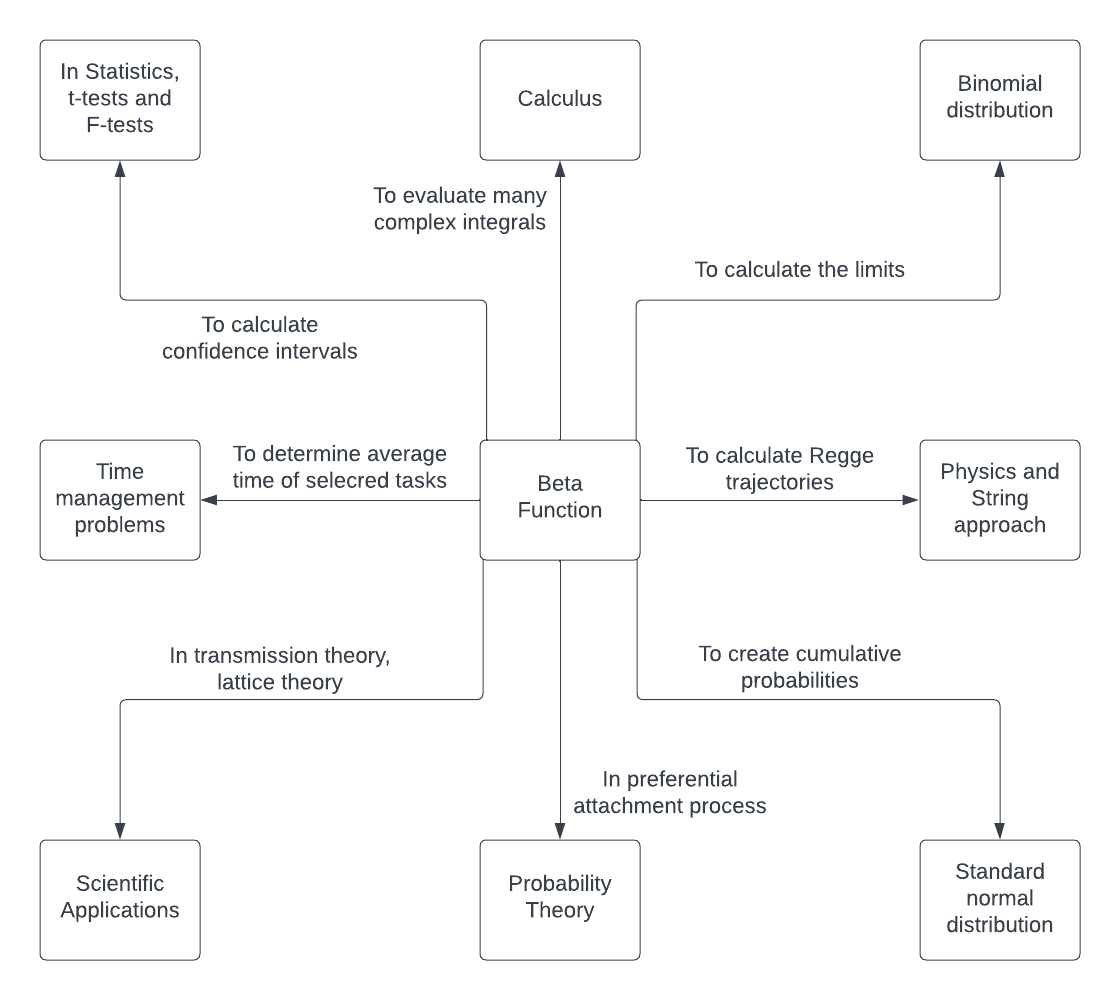
\includegraphics[width=1.0\linewidth]{Images/beta_contextmodel.png}    
    \end{center}
    \caption{Context of use model}
    \label{fig:Context of Use Model.}
\end{figure}



\chapter{Problem 2}
\section*{Assumptions}
    \begin{enumerate}[noitemsep]
        \item x and y are positive real numbers $x,y \in R^{+}$.
        \item It is simpler to calculate $B(x,y)$ using the factorial for $x,y \in Z^{+}$.
        \item If x and y are real numbers, there is no need to compute the integral function. The gamma values of the numbers may be used to derive the beta value using Stirling's approach.
    \end{enumerate}
\begin{enumerate}[noitemsep]
        \item \textbf{First Requirement}
        \begin{itemize}[noitemsep]
            \item \textbf{ID = } FR1
            \item\textbf{Type = } Functional Requirements
            \item\textbf{Version = } 1.0
            \item\textbf{Difficulty = } Easy
            \item\textbf{Description = } The Beta function $B(x,y)$ requires $x$ and $y$ as its two variable inputs in order to operate.
            \item\textbf{Rationalle = } $x$ and $y$ 
        \end{itemize}
        \item \textbf{Second Requirement}
        \begin{itemize}
            \item \textbf{ID = } FR2
            \item\textbf{Type = } Functional Requirements
            \item\textbf{Version = } 1.0
            \item\textbf{Difficulty = } Easy
            \item\textbf{Description = } The Beta function $B(x,y)$ requires two real positive numbers as it's defined in the $R^{+}$ domain.
            \item\textbf{Rationalle = } $x \geq 0$ and $y \geq 0$ 
        \end{itemize}
        \item \textbf{Third Requirement}
        \begin{itemize}
            \item \textbf{ID = } FR3
            \item\textbf{Type = } Functional Requirements
            \item\textbf{Version = } 1.0
            \item\textbf{Difficulty = } Easy
            \item\textbf{Description = } The Beta Value of the function is in real positive numbers i.e $R^{+}$
            \item\textbf{Rationalle = } $B(x,y) \geq 0$ 
        \end{itemize}
        
        \newpage
        \item \textbf{Fourth Requirement}
        \begin{itemize}
            \item \textbf{ID = } FR4
            \item\textbf{Type = } Functional Requirements
            \item\textbf{Version = } 1.0
            \item\textbf{Difficulty = } Easy
            \item\textbf{Description = } If the given inputs are positive integers then beta Values can be easily computed by using the Beta - Gamma Function relation.
            \item\textbf{Rationalle = } \{ $\forall x,y \in Z^{+} \mid B(x,y) = \frac{\Gamma x \Gamma y}{\Gamma (x+y)} $\}
        \end{itemize}
        \item \textbf{Fifth Requirement}
        \begin{itemize}
            \item \textbf{ID = } FR5
            \item\textbf{Type = } Functional Requirements
            \item\textbf{Version = } 1.0
            \item\textbf{Difficulty = } Moderate
            \item\textbf{Description = } To calculate Beta function for large integer values, Gamma Function should be used in order to prevent stack overflow by using tail recursive function.
            \item\textbf{Rationalle = } \{ $\forall x,y \in R^+ \mid B(x,y) = \frac{{\Gamma x} {\Gamma y}}{\Gamma (x+y)} \; where\; \Gamma n = (n-1)! $ \}
        \end{itemize}
        
        \item \textbf{Sixth Requirement}
        \begin{itemize}
            \item \textbf{ID = } FR6
            \item\textbf{Type = } Functional Requirements
            \item\textbf{Version = } 1.0
            \item\textbf{Difficulty = } Difficult
            \item\textbf{Description = } For the decimal number gamma value can be calculated using the stirlings's approximation which helps in determining the Beta value without using the integral functions.
            \item\textbf{Rationalle = } \{ $\forall x,y \in R^{+} \mid B(x,y) = \frac{{\Gamma x} {\Gamma y}}{\Gamma (x+y)}\;where\; \Gamma n = \sqrt{2 \cdot \pi \cdot n}\cdot (\frac{n}{e})^{n}$ \} 
        \end{itemize}
        
        \item \textbf{Seventh Requirement}
        \begin{itemize}
            \item \textbf{ID = } FR7
            \item\textbf{Type = } Functional Requirements
            \item\textbf{Version = } 1.0
            \item\textbf{Difficulty = } Moderate
            \item\textbf{Description = } There is no definition of beta values for negative or zero values. There shouldn't be any inputs besides the numeric values; x and y can be similar or different, but there shouldn't be any inputs other than the numeric values.
            \item\textbf{Rationalle = } $x \leq 0\;and\;y \leq 0,\;x = y \;or\; x \neq y \;where\; x,y \in  R^{+} $
        \end{itemize}
        \newpage
        
        \item \textbf{Eighth Requirement}
        \begin{itemize}
            \item \textbf{ID = } QR1
            \item \textbf{Type = } Non-Functional Requirement
            \item \textbf{Version = } 1.0
            \item \textbf{Difficulty = } Easy
            \item \textbf{Description = } The system should maintainable and changes can be easily applied to the system.
            \item \textbf{Rationalle = } The maintainability is provided by dividing distinct tasks into different modules or functions.
        \end{itemize}
        
        \item \textbf{Ninth Requirement}
        \begin{itemize}
            \item \textbf{ID = } QR2
            \item \textbf{Type = } Non-Functional Requirement
            \item \textbf{Version = } 1.0
            \item \textbf{Difficulty = } Easy
            \item \textbf{Description = } The system should be portable and able to run on different system such as various operating system.
            \item \textbf{Rationalle = } The Java (requires version 1.8 or above) programs are compatible with any system architecture that has a JVM (Java Virtual Machine).
        \end{itemize}
        
        \item \textbf{Tenth Requirement}
        \begin{itemize}
            \item \textbf{ID = } QR3
            \item \textbf{Type = } Non-Functional Requirement
            \item \textbf{Version = } 1.0
            \item \textbf{Difficulty = } Easy
            \item \textbf{Description = } The system design should be easy to understand for any user and can easily interpret the error message displayed on the system even for non-technical users.
            \item \textbf{Rationalle = } The error message should clearly state what went wrong.
        \end{itemize}
    \end{enumerate}


\chapter{Problem 3}
\section{Algorithm 1 - Tail Recursive Factorial Function}
The gamma function is utilised by the beta function to calculate positive integers. The factorial of the number makes it simple to determine the Gamma Value of a positive integer. 
\begin{center}
    $B(x,y)=\frac{\Gamma x \Gamma y}{\Gamma (x+y)}$ where $\Gamma x = (x-1)!$\\
\end{center}

\subsection{Advantages}
\begin{itemize}
    \item The algorithm Gives the accurate answers for the positive integers.
    \item The execution speed of the tail recursive function compared to recursive function is very fast and memory efficient. 
    \item This algorithm makes it simple to calculate the integer's beta values.
\end{itemize}
\subsection{disadvantages}
\begin{itemize}
    \item Can be used for only Positive numbers.
    \item Only calculate the Beta Values for the integer
    \item It does not Consider decimal numbers.
\end{itemize}

\subsection{Why Tail Recursive Function ?}
If a function concludes by returning the result of the recursive call, it is considered tail-recursive. It is a waste of memory to keep the caller's frame on the stack after the recursive call returns its value because nothing else has to be done. Therefore, the current frame can be used for the call rather than allocating a new one. And for the small value of the integer sometimes recursive factorial faction can cause StackOverFlow error that's why it's better to use the tail recursive function. \\

\newpage
\subsection{Algorithm}

\begin{algorithm}
\caption{Calculate Beta Function using factorial}

\textbf{Require:}  value: $x > 0$ \& $y>0$  \Comment{where $x,y \in {Z}^+$}\\
\textbf{Ensure:} $result = Beta(x,y)$
\begin{algorithmic}[1]

\Procedure {BetaFunction}{$x, y$}
    \State $value1 \leftarrow \Call{CalculateGamma}{x}$
    \State $value2 \leftarrow \Call{CalculateGamma}{y}$
    \State $value3 \leftarrow \Call{CalculateGamma}{x+y}$
    \State $betaValue \leftarrow \frac{value1 * value2}{value3}$
    \State \textbf{return} $betaValue$\Comment{It returns the beta value}
    \EndProcedure
\Statex


\Procedure {GammaFunction}{$value$}
    \State $value \leftarrow value-1$
    \State \textbf{return} $\Call{Factorial}{value}$ \Comment{It returns the gamma value}
    \EndProcedure
\Statex

\Procedure {Factorial}{$value$}
    \State \textbf{return} $\Call{FactorialTailRecursive}{value,1}$ \Comment{It returns the factorial of the number}
    \EndProcedure
\Statex

\Procedure{FactorialTailRecursive}{$value, n$}
    \If{$value = 0 $}
    \State \textbf{return} $n$ \Comment{Return factorial of the number} 
    \Else
    \State \textbf{return} \Call{FactorialTailRecursive}{$value - 1$, $value * n$ } \Comment{tail recursive call to function}
    \EndIf
    \EndProcedure
\Statex


\State $result \leftarrow \Call{CalculateBeta}{x,y} $\Comment{Final result of $Beta(x,y)$}

\end{algorithmic}
\end{algorithm}

\newpage
\section{Algorithm 2 - Stirling's approximation}
The gamma Stirling's approximation, also referred to as Stirling's formula is a mathematical approximation for factorials for decimal values and can be used to construct the beta function for decimal numbers. Since it is a good approximation, it delivers correct results even for small values of n. \\

\begin{center}
    $B(x,y)=\frac{\Gamma x \Gamma y}{\Gamma (x+y)}$ where, $\Gamma n = \sqrt{2 \pi n} \cdot (\frac{n}{e})^n$\\
\end{center}

\subsection{Advantages}
\begin{itemize}
    \item The algorithm Gives the answers for the positive real numbers.
    \item Most values that are available can be computed by the algorithm.
    \item It is possible to apply this approximation approach in place of the integration function to reduce the complexity of the code
\end{itemize}
\subsection{disadvantages}
\begin{itemize}
    \item The algorithm is unable to produce reliable answers.
    \item Although the complexity is decreased, the earlier algorithm is still substantially more difficult.
    \item The code cannot be easily debugged.
    \item The mismatch between the necessary and actual answers is much different for smaller values. However, the difference gets smaller as the size of the numbers grows.
\end{itemize}

\subsection{Why to use Stirling's Approximation ?}
To calculate the Beta value of the decimal number, it's hard to compute using the gamma's integral function. However, Stirlings' approximation can be applied to reduce the complexity. Even for small numbers, this is a good approximation procedure that yields accurate answers. The best outcome is always obtained through approximation. The comparison of Stirling's approximation and the factorial is provided below.

\begin{figure}[h]
    \centering
    \begin{center}
    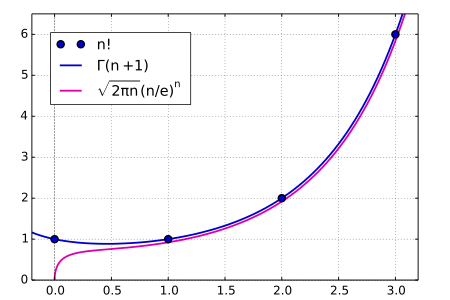
\includegraphics[width=0.39\linewidth]{Images/Mplwp_factorial_gamma_stirling.svg.png}    
    \end{center}
    \caption{Comparison of Stirling's approximation and the factorial. Source:-  \href{https://en.wikipedia.org/wiki/Stirling\%27s\_approximation}{WikiPedia}}
    \label{fig:OSI Layers Model.}
\end{figure}

\newpage
\subsection{Algorithm}

\begin{algorithm}
\caption{Calculate Beta Function using Stirlings's approximation}

\textbf{Require:}  value: $x > 0$ \& $y>0$  \Comment{where $x,y \in R^+$}\\
\textbf{Ensure:} $result = Beta(x,y)$
\begin{algorithmic}[1]

\Procedure {CalculateBeta}{$x, y$}
    \State $value1 \leftarrow \Call{CalculateGamma}{x}$
    \State $value2 \leftarrow \Call{CalculateGamma}{y}$
    \State $value3 \leftarrow \Call{CalculateGamma}{x+y}$
    \State $beta \leftarrow \frac{value1 * value2}{value3}$
    \State \textbf{return} $beta$\Comment{It returns the beta value}
    \EndProcedure
\Statex

\Procedure {CalculateGamma}{$value$}
    \State $firstPart \leftarrow 2 \cdot \pi \cdot value$
    \State $secondPart \leftarrow (\frac{value}{e})$
    \State $gamma \leftarrow \Call{CalculatePower}{firstPart,\frac{1}{2}} \Call{CalculatePower}{secondPart,value}$
    \State \textbf{return} $gamma$\Comment{It returns the gamma value}
    \EndProcedure
\Statex

\Procedure {CalculatePower}{$value1$,$value2$}
    \State $power \leftarrow math.power(value1,value2)$
    \State \textbf{return} $power$\Comment{It returns the base to the power}
    \EndProcedure
\Statex

\Procedure{CalculateLog}{$value$}
    \State $answer \leftarrow 0$
    \State $base \leftarrow \frac{value-1}{value+1}$
    \For {$i \leftarrow 1, 125 $}
    \State $exponent \leftarrow 2 * i - 1$
    \State $answer \leftarrow answer + \frac{1}{exponent}*\Call{calculatePower}{base,exponent}$
    \EndFor
    \State \textbf{return} $2*answer$ \Comment{It returns the value of Log n}
    \EndProcedure
\Statex
\State $result \leftarrow \Call{CalculateBeta}{x,y} $\Comment{Final result of $Beta(x,y)$}

\end{algorithmic}
\end{algorithm}

\begin{algorithm}
\caption{Calculate the power(x,y)}

\textbf{Require:}  value: $x$ \& $y$  \Comment{where $x,y \in R$}\\
\textbf{Ensure:} $result = Power(x,y)$
\begin{algorithmic}[1]

\Procedure {CalculatePower}{$base$,$exponent$}
    \State Convert the exponent into String
    \State $exponentArray \leftarrow Split\;the\;exponent\;into\;integer\;and\;fractional\;part$
    \If{$exponetArray[1] > 0$}
    \State \textbf{return} \Call{calculateFractionPower}{$base$,$exponent$}
    \EndIf
    %\State $value2 \leftarrow value-1$
    \If{$exponent < 0 $}
    \State $base \leftarrow \frac{1}{base}$
    \State $exponent \leftarrow (-1) \cdot exponent$
    \EndIf
    \If{$exponent \leftarrow 0$}
    \State \textbf{return} 1
    \EndIf
    \If{$exponent \% 2 \leftarrow 0$}
    \State $base \leftarrow base * base$
    \State $exponent \leftarrow \frac{exponent}{2}$
    \State \textbf{return} \Call{calculatePower}{$base$,$exponent$}
    \Else
    \State $exponent \leftarrow \frac{exponent-1}{2}$
    \State \textbf{return} $base$ * $\Call{calculatePower}{base*base,exponent}$
    \EndIf
    \EndProcedure
\Statex


\Procedure {CalculateFractionPower}{$base$,$exponent$}
    \State $answer \leftarrow 0$
    \State $logvalue \leftarrow 0$
    \If{$exponet \leftarrow 0$}
    \State \textbf{return} 1
    \EndIf
    \If{$base < 0 $}
    \State $logvalue \leftarrow \Call{calculateLog}{base * (-1)}$
    \Else
    \State $logvalue \leftarrow \Call{calculateLog}{base}$
    \EndIf
    \If{$exponent \leftarrow 0 \land exponent > 0$}
    \State \textbf{return} $answer$
    \EndIf
    \For {$i \leftarrow 0, 125 $}
    \State $numerator \leftarrow \Call{calculatePower}{exponent*logvalue,i}$
    \State $denominator \leftarrow \Call{Factorial}{i}$
    \State $answer \leftarrow answer + \frac{numerator}{denominator}$
    \EndFor
    
    \If{$base < 0 \land \;exponent \% 2 \neq 0$}
    \State \textbf{return} $answer * (-1)$
    \Else
    \State \textbf{return} $answer$
    \EndIf
    \EndProcedure
\Statex

\end{algorithmic}
\end{algorithm}

\newpage

\section{Mind Map}

\begin{figure}[h]
    \centering
    \begin{center}
    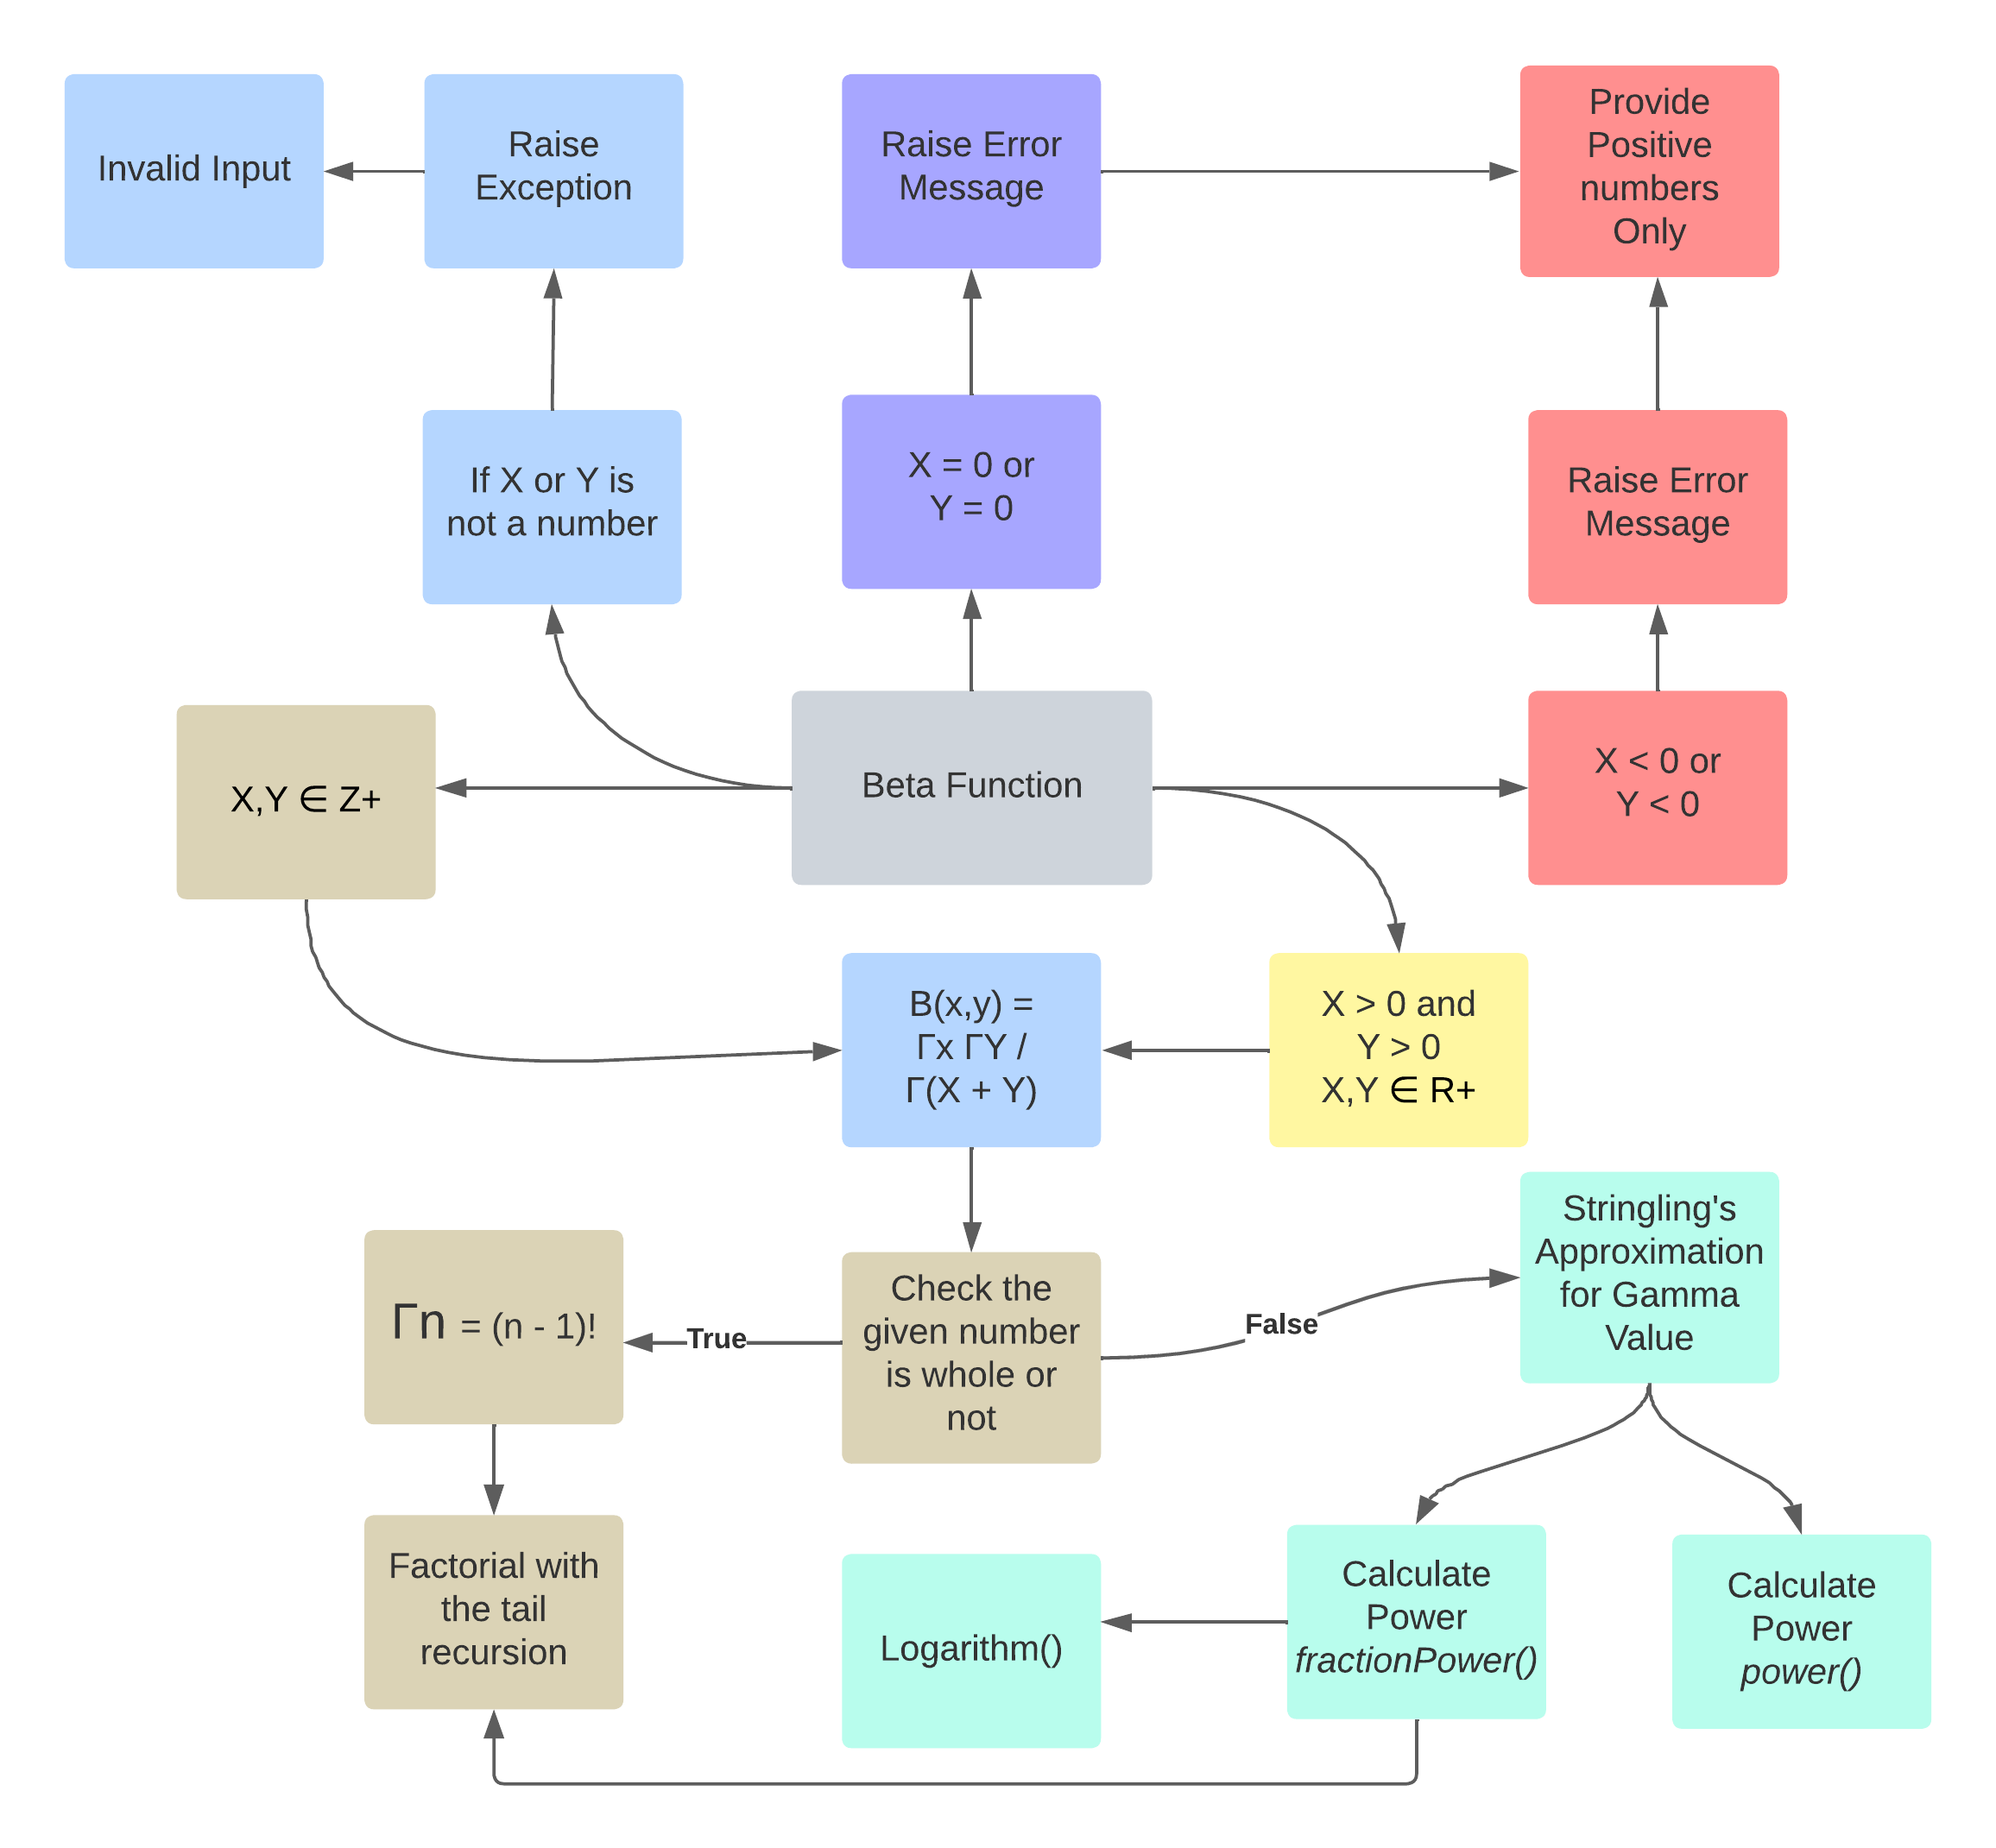
\includegraphics[width=1.0\linewidth]{Images/Mind-Map.png}    
    \end{center}
    \caption{Mind Map for Pseudo Code}
    \label{fig:Mind Map}
\end{figure}

\newpage

\chapter{Problem 4}

\section{Code Review for Function-6 Beta Function $B(x,y)$}
\subsection{Debugger}
A debugger is computer software or a tool that programmers use to test and debug a target program. By employing instruction-set simulators rather than running a program directly on the CPU, debuggers can exert more control over how it is executed. This makes it possible for debuggers to pause or terminate the application in response to specific events. In this case, the debugger tool of the Eclipse IDE is used to troubleshoot the code of the beta function calculator. Breakpoints are utilized to temporarily halt the execution of the code. \\
\subsubsection{Advantages}
    \begin{itemize}[noitemsep]
        \item Able to examine and analyse the values of a stack, heap, or variable at a single line of code.
        \item Can stop the program's execution at a specific moment to examine its path and its values with the help breakpoints.
        \item Can be easily applied to the running program.
    \end{itemize}
\subsubsection{Disadvantages}
     \begin{itemize}[noitemsep]
        \item Does not support real time and multi threading ahdoc
        \item May not able to expose all the problems
    \end{itemize}


\begin{figure}[h]
    \centering
    \begin{center}
    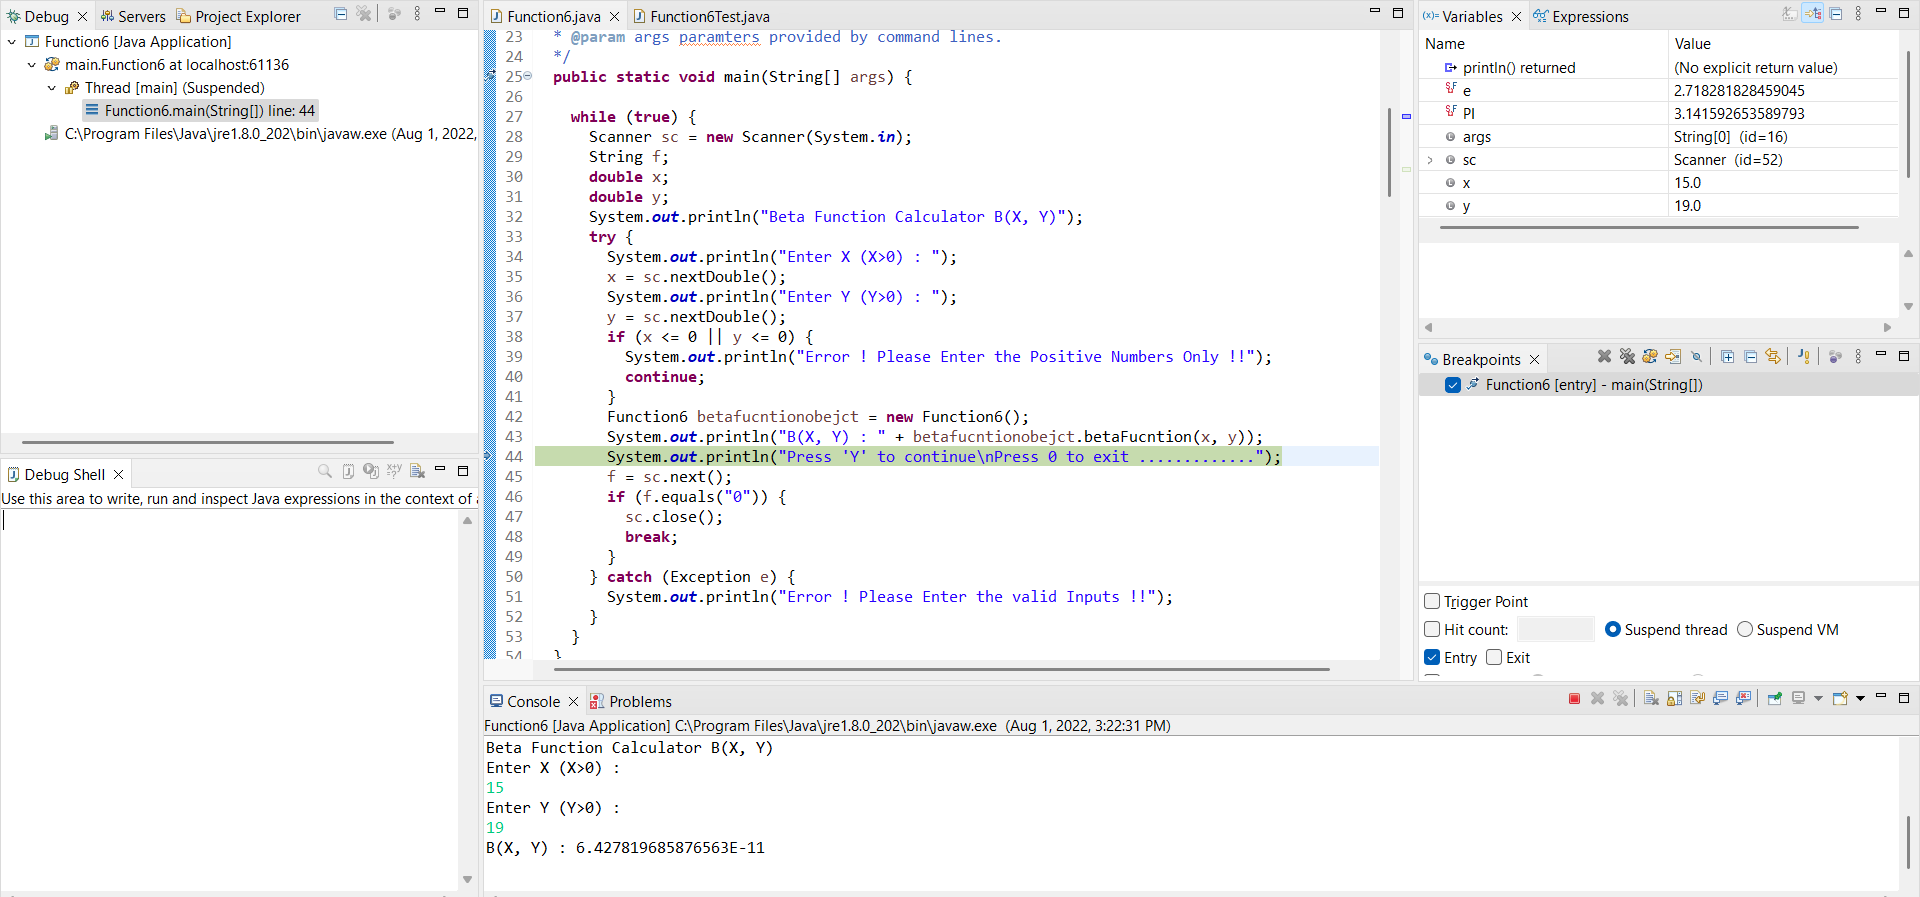
\includegraphics[width=0.73\linewidth]{Images/Debugger_snapshot.png}    
    \end{center}
    \caption{Snapshot of the Eclipse IDE debugger tool }
    \label{fig:Eclipse Debugger Tool snapshot.}
\end{figure}

\newpage
\section{CheckStyle Tool}
The "CheckStyle" plugin for Eclipse provides the code specifications and guarantees that the java code adheres to the accepted code styles. Java code for the beta function was validated using the Google check style. Following snapshot shows there is not any coding standard violations in the Beta Function code.\\
\subsubsection{Advantages}
    \begin{itemize}[noitemsep]
        \item Supports Automatic Checking and can be used in the ongoing project. automatically checks the coding standards line by line.
        \item Supports multiple types of check styles such as Google and Sun microsystems coding standards.
        \item CheckStyle tool is portable and can be used with any IDEs and help to unify the team across various boundaries.
    \end{itemize}

\subsubsection{Disadvantages}
    \begin{itemize}[noitemsep]
        \item To validate the coding standard, it needs to be re-compiled every time
        \item Only validate the code specification rather than apply the changes and modify them according to the given checkstyle specification.
        \item This tool has its flaws. needs to be refreshed or sometimes have to clean and build the project again to refrain from errors.
    \end{itemize}
    
\begin{figure}[h]
    \centering
    \begin{center}
    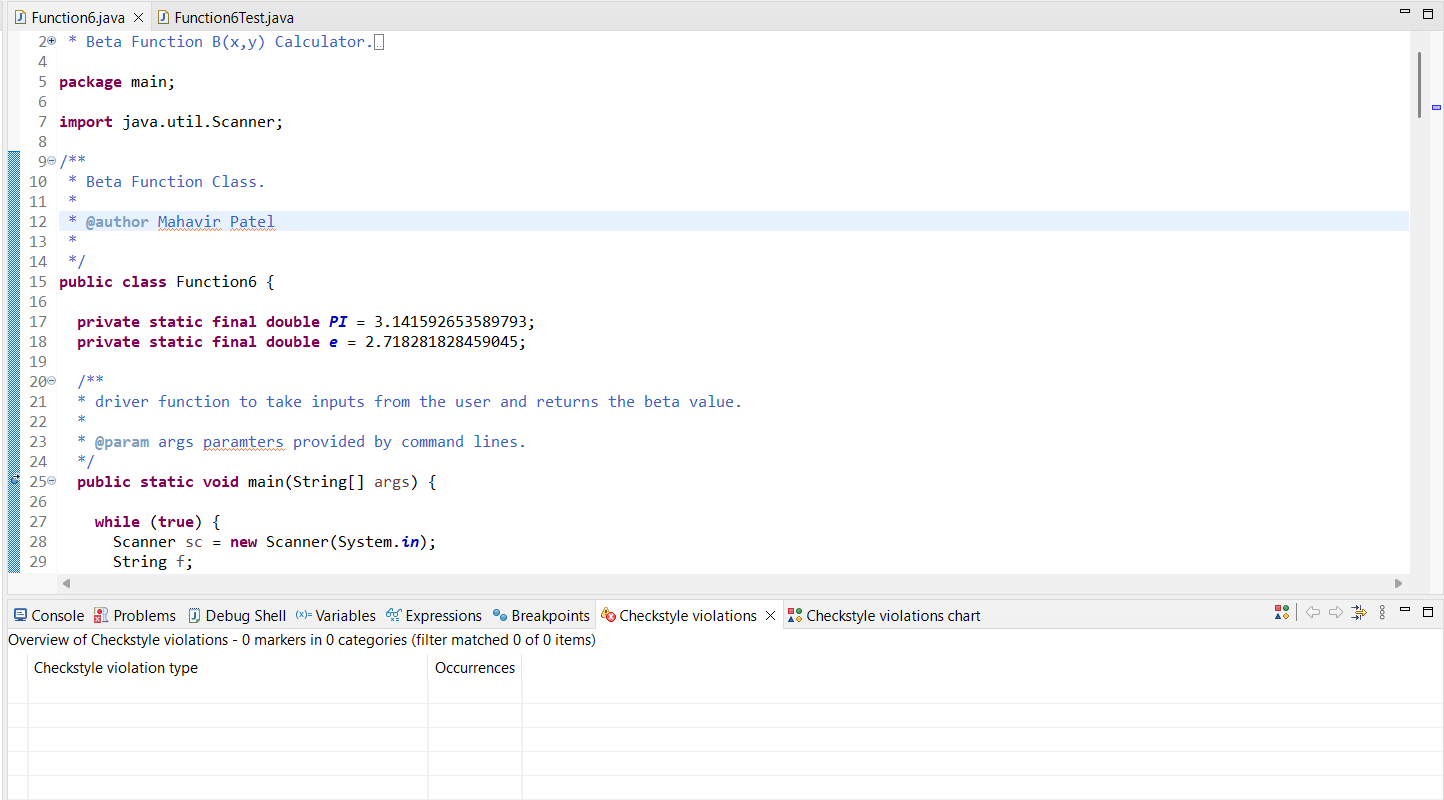
\includegraphics[width=1.0\linewidth]{Images/Checkstyle_tool_snapshot.png}    
    \end{center}
    \caption{Snapshot of the Eclipse CheckStyle plugin }
    \label{fig:Eclipse CheckStyle Plugin}
\end{figure}

\newpage
\section{PMD - Pragmatic Quality Tool}
PMD, or programming mistake detector is a source code analyzer. It detects typical programming errors such as unnecessary variables, empty catch blocks, It detects typical programming errors such as unnecessary variables, empty catch blocks, unneccesary object creation, etc. The code error seen in the following screenshot was found in Ecplise IDE's source code and was verified using the PMD plugin. \\ 
\subsubsection{Advantages}
    \begin{itemize}[noitemsep]
        \item By examining unnecessary variables or objects, space efficiency is increased and code analysis can be done.
        \item The copy-paste detector, or CPD, is offered. In the source code, redundant code is discovered.
        \item Multiple programming languages, markup languages, Salesforce.com Apex and Visualforce, PLSQL, Apache Velocity, XML, XSL, and other technologies are supported.
        \item Additionally PMD allows user-defined rules for source code analysis
    \end{itemize}
\subsubsection{Disadvantages}
    \begin{itemize}[noitemsep]
        \item There are times when these programmes generate false positives and false negatives, providing the appearance that everything is being addressed.
        \item Since it is more difficult to identify the precise location of the code vulnerability, a solution takes longer to implement. Vulnerabilities in the runtime environment are not found.
    \end{itemize}

\begin{figure}[h]
    \centering
    \begin{center}
    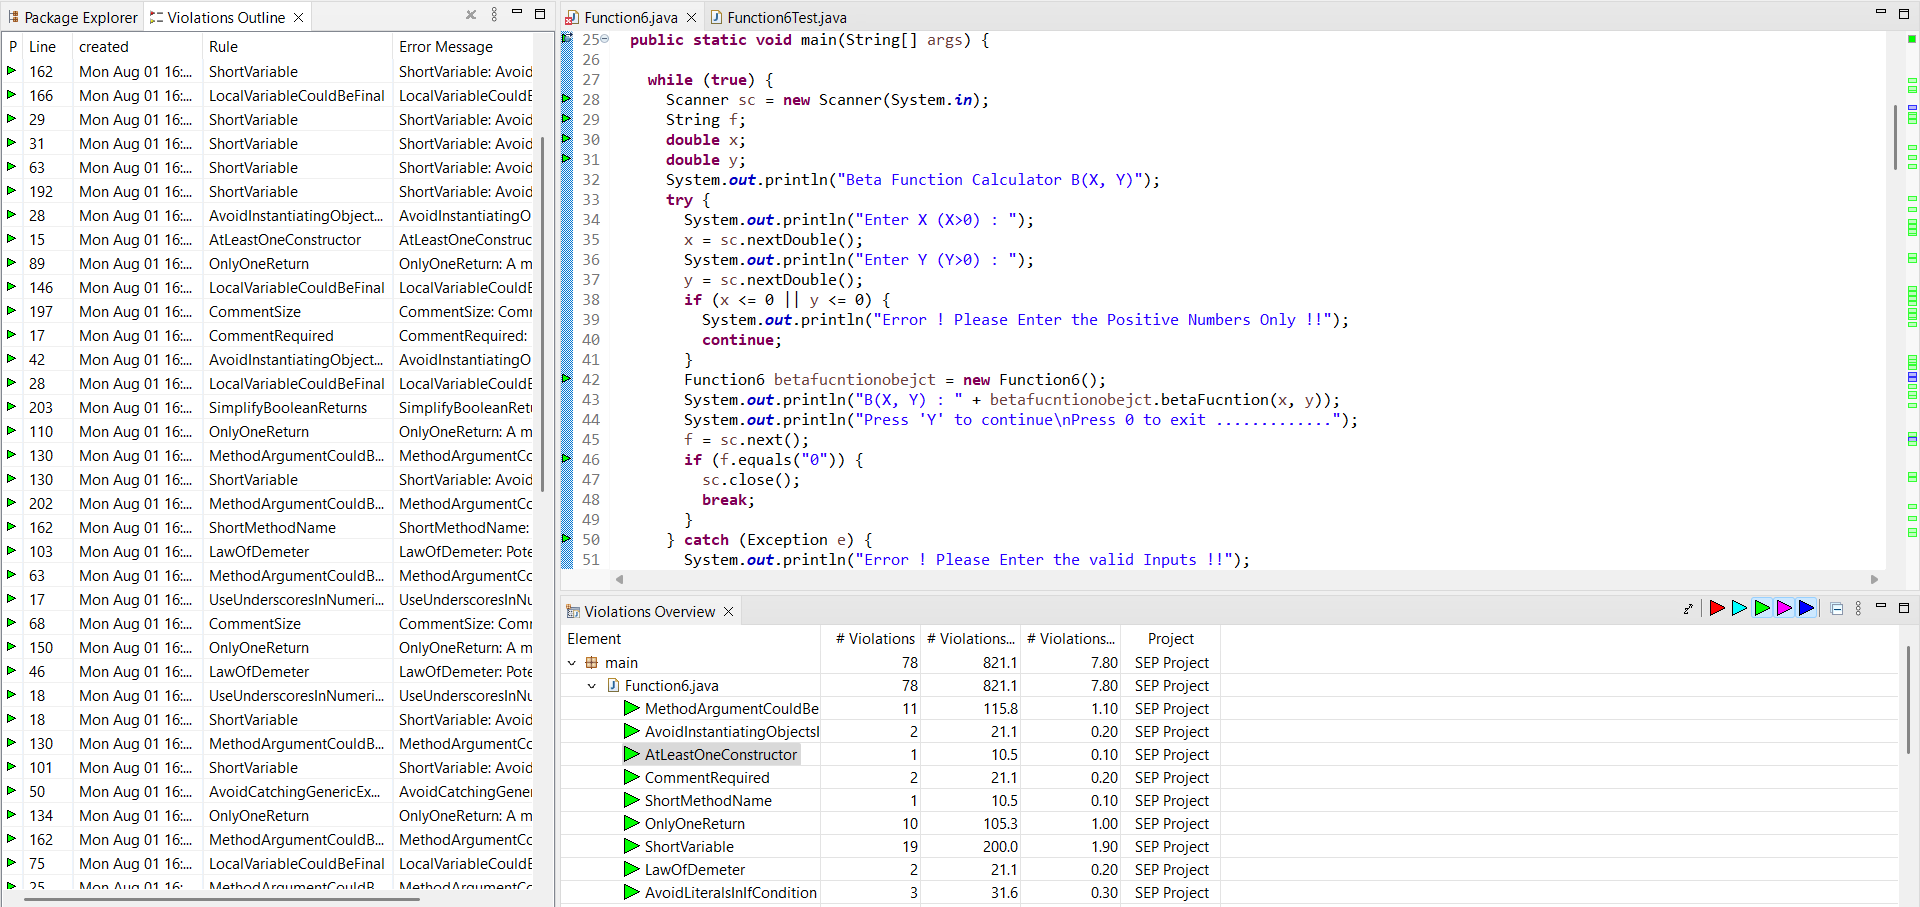
\includegraphics[width=1.0\linewidth]{Images/PMD_plugin_violations.png}    
    \end{center}
    \caption{Snapshot of the Eclipse PMD plugin}
    \label{fig:Eclipse PMD Plugin}
\end{figure}

\newpage

\section{Quality Attributes}
\subsection{Usability}
The beta function calculator has a straightforward user interface that is easy enough for non-technical people to understand. Additionally, it offers an error message that any user may readily understand, such as improper inputs or beta function values such as negative or zero. Even for small values of integers, the Stirlings Approximation offers the user confidence in the accuracy of the solution.
\subsection{Maintainability}
Due to the separation of various tasks, the beta function calculator is simple to maintain without causing any system disruptions or crashes. Additionally, the user interface might be included. Furthermore, it may be adjusted to account for changes in the future and can accommodate various approaches to determine the beta values of the inputs.
\subsection{Correctness}
The results from this calculator are correct for integer numbers. However, it delivers an accurate answer with an accuracy of up to 7 decimal places for fractional integers. Even with a small number, Stirling's approach produces almost exact results, but as the number increases, the method gives a user the right answers.
\subsection{Efficiency}
In both space and time, the calculator application is incredibly effective. It reduces the StackOverflow error using the tail recursive method and provides correct results in a short amount of time.
\subsection{Robustness}
The beta calculator is really reliable. It offers an error message that the user may readily understand. If invalid inputs are given, the program will continue to run without pausing the process and will give an error message based on the circumstances that led to the disruption in the flow.

\newpage
\section{Error Message and Exception Handling}
Responding to undesirable or unexpected events that occur while a computer program is running is known as exception handling. Without this procedure, exceptions would disrupt a program's normal operation and lead to a crash. To avoid this, exception handling deals with these occurrences.\\\\
In Beta Function Calculator, if a user enters a number other than positive real numbers, then the user will be notified by an error message "Please enter the positive numbers only"\\\\
Moreover, if the user enters a String as input then the system throws an exception containing a message "Please enter the valid inputs" and for any general exception a message "Fatal error" is thrown by an exception handling mechanism.

\newpage

\chapter{Problem 5}

\section*{Requirements Traceability}
Here given below is the JUnit test case report to check all the requirement has been satisfied.
\subsection*{1. Test Case}
    \begin{itemize}
        \item \textbf{Test Case ID : } TC1
        \item \textbf{Requirement ID : } FR1, FR2, FR3, FR7
        \item \textbf{Test Case Method : } testMain()
        \item \textbf{Description : } The testMain() function verifies if the user has supplied accurate and legitimate inputs. If not it will provide the Error message and handles the exception. It also check the inputs are not zero or negative or string or character. 
        \item \textbf{Test Inputs : }(9,9), (-4,-4), (-4,0), (1,3)
        \item \textbf{Test Expected Outcome : }4.570592805886924E-6, Error Message, Error Message, 0.3333333333333333
        \item \textbf{Test Actual Outcome : }4.570592805886924E-6, Error Message, Error Message,\\ 0.3333333333333333 
        \item \textbf{Result : }Success
    \end{itemize}

\subsection*{2. Test Case}
    \begin{itemize}
        \item \textbf{Test Case ID : } TC2
        \item \textbf{Requirement ID : } FR4, FR5, FR7
        \item \textbf{Test Case Method : } testBetaFunction()
        \item \textbf{Description : } The testBetaFunction() checks the inputs and and calculate the beta values with the help of gamma beta function relation. 
        \item \textbf{Test Inputs : }(1,1), (100,1)
        \item \textbf{Test Expected Outcome : }1, 0.009999999999999998
        \item \textbf{Test Actual Outcome : }1, 0.009999999999999998 
        \item \textbf{Result : }Success
    \end{itemize}

\subsection*{3. Test Case}
    \begin{itemize}
        \item \textbf{Test Case ID : } TC3
        \item \textbf{Requirement ID : } FR4, FR6
        \item \textbf{Test Case Method : } testBetaFunctionFraction()
        \item \textbf{Description : }The testBetaFunctionFraction() calculate the beta values for the fractional numbers using the stirling's approximation because  the factorial of the decimal number is not defined.
        \item \textbf{Test Inputs : }(15.8, 20.8)
        \item \textbf{Test Expected Outcome : }1.1488056591230658E-11
        \item \textbf{Test Actual Outcome : }1.1488056591230658E-11
        \item \textbf{Result : }Success
    \end{itemize}

\subsection*{4. Test Case}
    \begin{itemize}
        \item \textbf{Test Case ID : } TC4
        \item \textbf{Requirement ID : } FR7
        \item \textbf{Test Case Method : } testBetaFunctionZero()
        \item \textbf{Description : }The testBetaFunctionFraction() check the error message and validate the exception if one the input value is zero.
        \item \textbf{Test Inputs : }(0,0), (0,5), (5,0)
        \item \textbf{Test Expected Outcome : }Exception and Error Message
        \item \textbf{Test Actual Outcome : }Exception and Error Message 
        \item \textbf{Result : }Success
    \end{itemize}
    
\subsection*{5. Test Case}
    \begin{itemize}
        \item \textbf{Test Case ID : } TC5
        \item \textbf{Requirement ID : } FR7
        \item \textbf{Test Case Method : } testBetaFunctionNegative()
        \item \textbf{Description : }The testBetaFunctionNegative() check if the negative number is provided then the function does not stop and exception are handled properly. 
        \item \textbf{Test Inputs : }(-5,-5), (0,-5), (-5,0)
        \item \textbf{Test Expected Outcome : }Exception and Error Message
        \item \textbf{Test Actual Outcome : }Exception and Error Message 
        \item \textbf{Result : }Success
    \end{itemize}
    
\subsection*{6. Test Case}
    \begin{itemize}
        \item \textbf{Test Case ID : } TC6
        \item \textbf{Requirement ID : } FR4, FR5
        \item \textbf{Test Case Method : } testWholeNumber()
        \item \textbf{Description : }The test method testWholeNumber() checks the given inputs is whole number or the fraction.  
        \item \textbf{Test Inputs : }0.12, 789.646, 12.00, 45
        \item \textbf{Test Expected Outcome : }False, False, True, True
        \item \textbf{Test Actual Outcome : }False, False, True, True 
        \item \textbf{Result : }Success
    \end{itemize}

\begin{thebibliography}{15}

\addcontentsline{toc}{chapter}{Bibliography}
\bibitem{1}
Beta Function WikiPedia
\\\href{https://en.wikipedia.org/wiki/Beta\_function}{https://en.wikipedia.org/wiki/Beta\_function}

\bibitem{2}
Beta Function Properties
\\\href{https://byjus.com/maths/beta-function/}{https://byjus.com/maths/beta-function/}

\bibitem{3}
Stirling's Approximation
\\\href{https://en.wikipedia.org/wiki/Stirling\%27s\_approximation}{https://en.wikipedia.org/wiki/Stirling\%27s\_approximation}

\bibitem{4}
Tail Recursion
\\\href{https://www.geeksforgeeks.org/tail-recursion/}{https://www.geeksforgeeks.org/tail-recursion/}

\bibitem{5}
Error Handling Defination
\\\href{https://www.techtarget.com/searchsoftwarequality/definition/error-handling}{https://www.techtarget.com/searchsoftwarequality/definition/error-handling}

\bibitem{6}
PMD
\\\href{https://pmd.github.io/latest/index.html}{https://pmd.github.io/latest/index.html}

\bibitem{7}
Debugging in the Eclipse IDE
\\\href{eclipse.org/community/eclipse\_newsletter/2017/june/article1.php}{eclipse.org/community/eclipse\_newsletter/2017/june/article1.php}

\bibitem{8}
Quality attributes in software architecture
\\\href{https://syndicode.com/blog/12-software-architecture-quality-attributes/}{https://syndicode.com/blog/12-software-architecture-quality-attributes/}

\bibitem{9}
Google's Software Architecture and Quality Attributes
\\\href{https://sites.google.com/site/misresearch000/home/software-architecture-quality-attributes}{https://sites.google.com/site/misresearch000/home/software-architecture-quality-attributes}

\bibitem{10}
Google Checkstyle for JAVA 
\\\href{https://checkstyle.sourceforge.io/google\_style.html}{https://checkstyle.sourceforge.io/google\_style.html}




\end{thebibliography}

\end{document}
